\section*{Conclusion}

This technology gives possibilities in developpement to warehouses for adding drone carriers around sensible objects or animals.

\subsubsection{Limits and Future Work}

As discussed previously in the paper, the current platform has some limitations that need to be addressed in future work. One of the main limitations is the reliance on lighthouse technology \cite{noauthor_dvic_nodate} for positioning. While it uses sensors that are effective, they are light sensitive  and may not be suitable for all indoor environments especially close to windows. Future work will focus on developing arount a more robust location system that can adapt to different environments and scenarios.

There is also a need to provide a cybersecurity layer to the platform to ensure that the drones are secure from external threats. This will involve developing a secure communication protocol to protect the drones from unauthorized access.

Finaly the platform needs to be tested in a real-world environment to evaluate its performance and reliability. This will involve conducting experiments in different indoor environments to assess the platform's intuitiveness against students. The results of these experiments will help to identify any issues with the platform and guide future development efforts.

\pagebreak

\appendix
\section{Pose etimation pipeline.}\label{appendix:additional_work}

\begin{figure}[htbp]
    \centerline{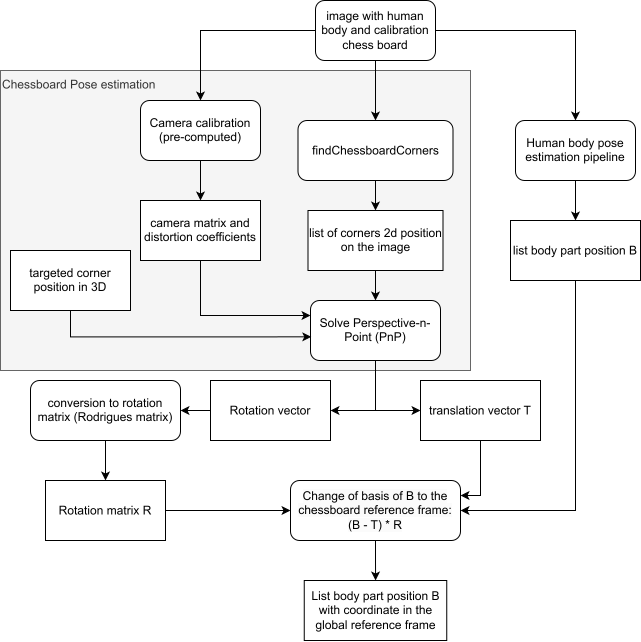
\includegraphics[width=0.5\textwidth]{images/objectcomplete.png}}
    \caption{Object Control Kernel, inside logics.}
    \label{fig}
    \end{figure} 
    The system leverages pose estimation to detect human body landmarks using computer vision, specifically OpenCV's pose estimation pipeline. First, a camera captures RGB and depth data from the environment, with the depth data being crucial for calculating the distance of each detected point. The system uses a monocular camera setup, and it processes images through MediaPipe's holistic model, which detects human body landmarks, including key body joints like the head, shoulders, and limbs. These 2D landmarks are then projected into 3D space using depth data from the RealSense camera.

    The system performs camera calibration to compute intrinsic parameters such as the camera matrix and distortion coefficients. Calibration ensures that the system accurately maps 2D pixel coordinates to real-world 3D points. OpenCV’s solvePnP function computes the human's pose (rotation and translation vectors) relative to the camera using chessboard patterns, which serve as a known reference in the scene. After obtaining the pose, the Rodrigues rotation matrix is used to transform the body landmarks into the coordinate system of the chessboard, essentially re-aligning the 3D positions of the detected human body with the physical world.
    
    This process ensures that the system can track human movement in 3D space accurately, which is crucial for human-drone interaction and control.

\pagebreak

\section*{Acknowledgment}
A Testbed Environment for Task Development was developed at
the IFT. Marc Teyssier, Xiao Xiao and Clement Duhart showed
much faith to enable such a project.

Etienne Pommel and Maximilien Menesguen of the Institute for future technologies, thank you
for joining yourselves to me. Your enthusiasm and dedication to the project have been a great source of inspiration.

Thomas Carstens and Nicolas Stas of the Institute for future technologies have been a great help in the development of the platform. Your technical expertise and guidance have been invaluable.
